\documentclass[11pt]{article}
\usepackage[review]{acl}
\usepackage{times}
\usepackage{latexsym}
\usepackage[T1]{fontenc}
\usepackage[utf8]{inputenc}
\usepackage{microtype}
\usepackage{inconsolata}
\usepackage{graphicx}
\usepackage{booktabs}
\usepackage{amsmath}
\usepackage{url}
\usepackage{multirow}

\title{When Do Member-Derived Embeddings Represent Labels? Evidence from Educational Knowledge Components}

\author{Anonymous EMNLP Submission}

\begin{document}
\maketitle
\begin{abstract}
NLP systems often represent labels or categories by embedding their names, descriptions, or member examples. We study a focused variant: representing a category by aggregating embeddings of the instances assigned to it. Educational Knowledge Components (KCs) provide a useful test case because each KC is a human-defined label over many question texts, but also acts as a functional state variable in knowledge tracing. Across ASSISTments datasets, member-derived KC prototypes recover substantial category signal: mean-prototype Recall@1 is 0.833, compared with 0.017 under shuffled prototypes, and heuristic label alignment reaches mean NMI 0.570. However, downstream functionality is mixed or weak. Prototype graphs align weakly with KT functional graphs, difficulty prediction has negative mean $R^2$, and Chapter 5 DKT initialization does not reliably improve over learned interaction embeddings. Transition prediction is the main positive diagnostic, but it does not rescue the stronger DKT result. We argue that member-derived label representations require downstream validation: recovering label membership is not sufficient evidence that an embedding is a useful functional prior.
\end{abstract}

\section{Introduction}
Many NLP systems need a representation for a label. In some settings the label is represented by its name, by a natural-language definition, by a prompt, or by a small set of examples. This paper studies a simple but consequential case: a category is represented by aggregating embeddings of the instances assigned to it. We call these \emph{member-derived label representations}. Such representations are attractive because they require no new annotation beyond category membership. They are also risky: high semantic similarity among members may not imply that the resulting vector is useful for a downstream task.

We examine this risk through educational Knowledge Components (KCs). A KC is a human-defined label over educational questions, such as a math skill or concept. Each KC has member question texts, so a natural representation is the mean, median, medoid, or otherwise aggregated embedding of those questions. At the same time, KCs are not merely topical labels. In knowledge tracing (KT), they define the sequence of student--skill interactions used to predict future correctness. This dual role makes KCs a useful testbed for label representation: we can ask whether a representation recovers category membership, and separately whether it captures the functional structure needed by a predictive model.

The paper is motivated by a negative downstream result from Chapter 5 of the thesis. That chapter tested text-derived KC-response embeddings as initializations for Deep Knowledge Tracing (DKT; \citealp{piech2015dkt}). Across nine construction pipelines, semantic/category initialization did not reliably improve DKT over the standard learned interaction embedding. We reframe that result as an NLP label-representation problem. The relevant question is not whether text embeddings are ``good'' or ``bad'' in general. The question is whether a representation obtained from constituent members is valid for the function assigned to the label.

This short paper makes a focused point. Member-derived KC representations encode category information, but category validity is not the same as downstream functional validity. We show that prototypes strongly recover KC membership and partially align with heuristic label groupings. However, their alignment with functional KT graphs is weak, and Chapter 5 downstream initialization results remain mixed or negative. The contribution is therefore a scoped negative finding: member aggregation is a reasonable way to represent labels for category recovery, but it should not be assumed to produce a functional prior without task-specific evidence.

Our contributions are:
(1) we formalize KCs as human-defined text labels for studying member-derived label representation;
(2) we evaluate category recovery, category coherence, heuristic label alignment, functional graph alignment, difficulty prediction, and transition prediction;
(3) we consolidate Chapter 5 downstream DKT evidence as the main functional test; and
(4) we identify failure modes that explain why an embedding can represent category membership while failing as a KT initialization.

\section{Related Work}
\paragraph{Label and category representation.}
NLP models often use labels as more than output IDs. Labels can be embedded from their names, expanded with descriptions, matched to examples, or treated as prompts. Weakly supervised and zero-shot classifiers use label semantics to connect text instances to categories, while prototype-based methods represent a class by one or more vectors estimated from examples \citep{snell2017prototypical,reimers2019sentencebert,meng2020lotclass}. Our setting is closest to example-derived category representation: the label vector is induced from constituent members rather than from the label name alone. The distinction matters because a member-derived representation can be evaluated both as a category prototype and as a downstream model component.

\paragraph{Similarity and downstream validity.}
Embedding similarity is not a single universal relation. Two texts may be similar by topic, reasoning step, difficulty, prerequisite relation, or expected student response pattern. Recent evaluation work in representation learning emphasizes that similarity should be tied to the target relation being modeled rather than treated as a generic property. Our study operationalizes that point: KC prototypes are tested against category membership and label-name structure, then separately against KT-relevant functional graphs and downstream DKT performance.

\paragraph{Educational text and knowledge tracing.}
Educational NLP has shown that question text can support tasks such as difficulty prediction, content tagging, and feedback generation. KT models, however, are trained on student interaction sequences and depend on temporal and behavioral regularities as much as text content. DKT \citep{piech2015dkt} represents each KC-response pair as an input symbol whose embedding is learned for prediction. Chapter 5 of the thesis replaces this learned initialization with text-derived KC-response embeddings and finds little robust improvement. Chapter 6 studies a different problem, redefining or reclustering the KC space itself; that direction is treated here only as separate work, not as evidence for the present paper.

\section{Data}
We use ASSISTments 2009, 2012, and 2017. Each dataset contains student interaction sequences and human-authored KC labels. We combine these with question--KC mapping files, Problem Bodies question text, and existing question-embedding artifacts in the repository. The embedding set includes sentence-transformer variants and available fine-tuned BERT embeddings; all analyses reuse existing artifacts rather than retraining KT models.

\begin{table}[t]
\centering
\small
\begin{tabular}{lrrrr}
\toprule
Dataset & Qs & Text Qs & KCs & Text KCs \\
\midrule
2009 & 26,688 & 7,836 & 123 & 76 \\
2012 & 179,999 & 32,792 & 265 & 162 \\
2017 & 3,162 & 638 & 102 & 68 \\
\bottomrule
\end{tabular}
\caption{Problem Bodies text coverage used by Chapter 5. Text linkage is incomplete, so member-derived label representations are available only for the text-linked subset.}
\label{tab:coverage}
\end{table}

Text linkage is a central constraint. Table~\ref{tab:coverage} shows that only 18--29\% of questions have the text linkage needed for the Chapter 5 initialization setting, although the linked KCs cover a larger share of the KC inventory. This matters for interpretation: our category-representation analyses test the subset where member question text is available, not every interaction in the KT benchmarks.

We report all generated metrics with dataset, embedding model, prototype method, metric name, unit of analysis, sample size, and source artifact path. When exact recomputation from raw artifacts is not possible, we mark values as thesis-text anchors from Chapter 5 rather than treating them as newly estimated results.

\section{Methods}
\paragraph{Member-derived KC representations.}
Let $q_i$ be a question text assigned to KC $c$, and let $e(q_i)$ be its embedding. A member-derived representation for $c$ is an aggregation over $\{e(q_i): q_i \in c\}$. We instantiate this with mean, median, and medoid prototypes where artifacts permit. Mean prototypes are the primary condition because they correspond directly to the common class-prototype assumption: a category can be summarized by the central tendency of its members.

\paragraph{Category-validity analyses.}
We first test whether prototypes recover the human KC labels. For each question, we retrieve the nearest KC prototype and compute Recall@1, Recall@5, MRR, NDCG, and a shuffled-prototype control. This is an optimistic diagnostic when the queried question contributes to its own KC prototype, so we interpret it as a category-signal check rather than a deployable classifier. We also measure coherence by comparing intra-KC and inter-KC cosine similarity and recording cluster diagnostics. Finally, we test whether prototype geometry aligns with coarse label information extracted heuristically from KC names. Because explicit curriculum metadata are incomplete, these label-alignment results are treated as weak supervision rather than gold taxonomies.

\paragraph{Functional analyses.}
Category recovery does not establish functional validity. We therefore evaluate three non-DKT downstream functionalities before the DKT initialization test. First, we compare prototype similarity graphs with KT-relevant graphs: transition relations, co-occurrence, difficulty similarity, and available DKT-derived KC relation artifacts. Second, we predict item difficulty from representations, treating difficulty as a psychometric functionality that a useful educational label representation might encode. Third, we predict KC transitions, treating next-KC structure as a sequential functionality of the label space. These diagnostics are not substitutes for DKT, but they test whether the representations encode behavioral structure beyond label membership.

\paragraph{Chapter 5 downstream test.}
The main downstream evidence is Chapter 5. DKT consumes KC-response inputs, so Chapter 5 constructs response-specific embeddings through nine pipelines. The pipelines vary whether question text is aggregated into KCs before adding response state, whether response state is added before aggregation, and whether KC-level or question-level text windows are used. We consolidate four Chapter 5 result families: full-data DKT initialization, reduced-data DKT initialization, fine-tuned BERT initialization, and post hoc alignment between semantic KC graphs and DKT-derived KC graphs. This paper treats those experiments as the decisive test of whether member-derived category representations become useful functional priors.

\section{Results}
\begin{figure}[t]
\centering
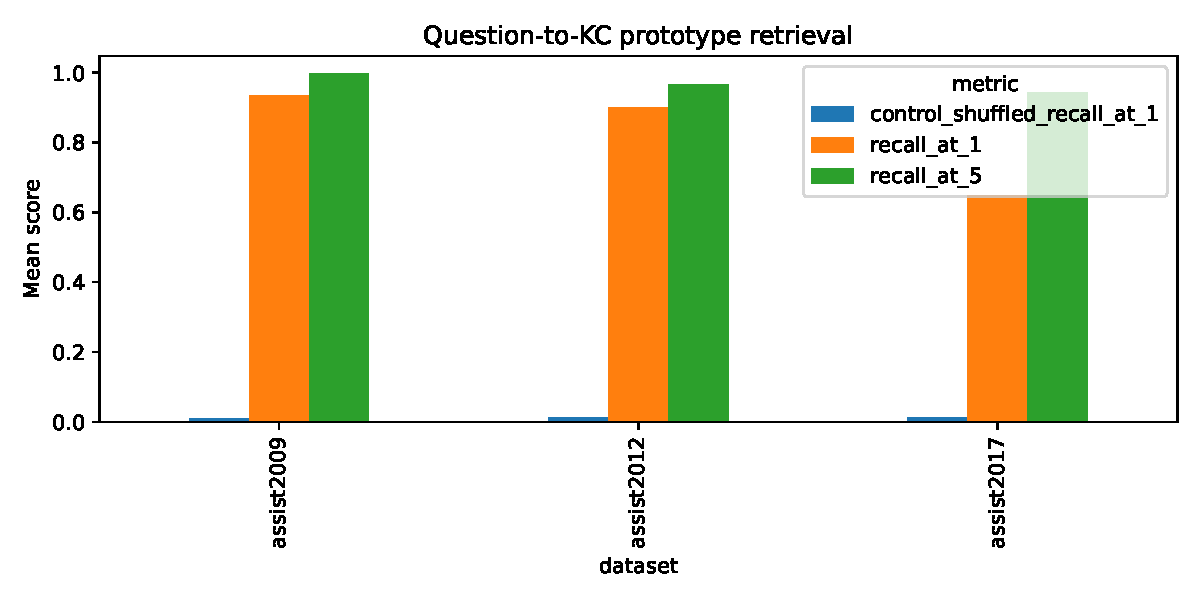
\includegraphics[width=\linewidth]{figures/fig2_prototype_retrieval.pdf}
\caption{Question-to-KC retrieval from member-derived prototypes. Prototypes recover category membership far above shuffled controls, showing that the representations contain real label information.}
\label{fig:retrieval}
\end{figure}

\begin{table}[t]
\centering
\small
\begin{tabular}{lrr}
\toprule
Analysis & Metric & Mean \\
\midrule
Retrieval & Recall@1 & 0.625 \\
Mean prototypes & Recall@1 & 0.833 \\
Shuffled control & Recall@1 & 0.017 \\
Retrieval & MRR & 0.707 \\
KC coherence & Intra--inter margin & 0.356 \\
Label alignment & NMI & 0.570 \\
Functional alignment & Spearman & 0.063 \\
Difficulty prediction & $R^2$ & -0.208 \\
Transition prediction & AUROC & 0.989 \\
Transition ranking & Recall@10 & 0.124 \\
\bottomrule
\end{tabular}
\caption{Summary of category and functional diagnostics. Retrieval and label-alignment metrics show category signal, but functional graph alignment is weak.}
\label{tab:diagnostics}
\end{table}

\paragraph{Member-derived prototypes recover KC membership.}
Figure~\ref{fig:retrieval} and Table~\ref{tab:diagnostics} show strong category recovery. Across prototype variants, Recall@1 averages 0.625, while shuffled prototypes average 0.017. Mean prototypes are stronger, with Recall@1 of 0.833 across 35 rows. MRR averages 0.707. These results support the first part of the story: aggregating member-question embeddings creates a meaningful representation of the human KC label.

\paragraph{The category signal is partial and heterogeneous.}
KC coherence is positive on average, with an intra-minus-inter cosine margin of 0.356 across 2,925 KC-level rows. However, the spread across KCs is important. Some KCs are compact text categories, while others combine heterogeneous problem forms under a single educational label. Heuristic label alignment is also partial: NMI averages 0.570 across 35 rows, but the label source is derived from KC names rather than a complete curriculum taxonomy. Thus the prototypes encode meaningful category information, but not a clean universal taxonomy.

\begin{table}[t]
\centering
\small
\begin{tabular}{p{0.26\linewidth}p{0.20\linewidth}p{0.42\linewidth}}
\toprule
Functionality & Result & Interpretation \\
\midrule
Functional graph alignment & $\rho=0.063$ & Prototype geometry weakly matches KT transition, co-occurrence, difficulty, and DKT-style graphs. \\
Difficulty prediction & $R^2=-0.208$ & Representations do not reliably encode item difficulty across datasets. \\
Transition prediction & AUROC $=0.989$; R@10 $=0.124$ & Representations/features can separate observed from unobserved transitions, but ranking exact next-KC edges remains modest. \\
DKT initialization & no full-data AUC gains & The strongest downstream test remains negative or mixed. \\
\bottomrule
\end{tabular}
\caption{Downstream functionality tests for member-derived KC label representations. The non-DKT diagnostics add nuance, but the main functional-prior claim is constrained by the DKT result.}
\label{tab:functionalities}
\end{table}

\paragraph{Other downstream functionalities are mixed.}
Table~\ref{tab:functionalities} expands the downstream evidence beyond DKT. The strongest contrast is between category recovery and functional alignment. Prototype geometry aligns only weakly with KT-relevant graph structure: mean Spearman correlation is 0.063 over 80 non-missing rows in the functional-structure table. By graph type, transition and co-occurrence alignments are positive but small (0.189 and 0.232), existing KC-graph alignment is near zero (0.048), and difficulty-similarity alignment is negative (-0.225). This suggests that category prototypes do not recover a stable functional relation over KCs.

Difficulty prediction is also weak in this run. Across 92 rows, mean $R^2=-0.208$, with ASSISTments 2012 below zero on average (-0.403) and ASSISTments 2017 near zero (0.004). Rank correlations are positive but modest: mean Spearman is 0.216 overall, 0.154 for 2012, and 0.283 for 2017. Thus the representations contain some difficulty-related signal, but not enough for reliable predictive functionality.

Transition prediction is the most positive non-DKT diagnostic. AUROC averages 0.989 and AUPRC averages 0.836, indicating that representation-derived features separate observed from unobserved transitions. However, ranking exact outgoing edges is much weaker: Recall@1 is 0.012 and Recall@10 is 0.124. We therefore treat transition prediction as evidence that the representations encode some sequential structure, not as evidence that they provide a complete functional KT prior.

\begin{table}[t]
\centering
\small
\begin{tabular}{lrrr}
\toprule
Dataset & Low-data $\Delta$AUC & BERT $\Delta$AUC & Best graph $r$ \\
\midrule
2009 & +0.0004 & +0.0029 & 0.0573 \\
2012 & +0.0002 & +0.0001 & 0.0894 \\
2017 & +0.0096 & -- & 0.0247 \\
\bottomrule
\end{tabular}
\caption{Chapter 5 DKT anchors. Reduced-data and fine-tuned BERT gains are small or inconsistent, and post hoc alignment between semantic KC graphs and DKT-derived KC graphs is weak.}
\label{tab:ch5}
\end{table}

\paragraph{DKT remains the main negative downstream result.}
Table~\ref{tab:ch5} summarizes the Chapter 5 evidence most relevant to this paper. In the full-data benchmark, no semantic/category initialization variant exceeds baseline test AUC on any dataset in the combined thesis comparison. Reduced-data results are mixed: mean $\Delta$AUC is +0.0004 for 2009, +0.0002 for 2012, and +0.0096 for 2017. Fine-tuned BERT makes initialization more competitive but produces only small gains, +0.0029 on 2009 and +0.0001 on 2012. The post hoc graph analysis points in the same direction: best Pearson correlations between semantic KC graphs and DKT-derived KC graphs are 0.0573, 0.0894, and 0.0247.

Taken together, the downstream functionality results sharpen the interpretation of Chapter 5. The representations are not functionally empty: transition diagnostics are strong under binary discrimination, and difficulty correlations are sometimes positive. But these signals are partial. They do not produce robust graph alignment, reliable difficulty prediction, or better DKT initialization. The downstream result is therefore not that text embeddings contain no information. It is that member-derived semantic/category representations are not reliable all-purpose functional representations of KCs.

\section{Discussion}
The results separate two senses of ``representing a label.'' In the category-recognition sense, the member-derived KC vectors work: they retrieve member questions, produce positive coherence margins, and partially align with label-name groupings. In the downstream functional sense, they are uneven. They show some transition-prediction signal, weak difficulty signal, weak graph alignment, and no reliable DKT initialization gain. The same vector can therefore be a reasonable category representation, a useful feature for some auxiliary functionality, and still a poor functional prior for the central KT model.

This distinction matters beyond education. Member aggregation is common because it is simple and intuitive: if a label is defined by its examples, average the examples. But a downstream model may need a relation that is not the same as topical similarity. For KCs, DKT benefits from structure about student trajectories, correctness patterns, skill dependencies, and dataset-specific sequencing. A question about two-step linear equations and a question about simplifying expressions may be textually similar, but their role in a student's learning path can differ. Conversely, two KCs may be functionally related because students transition between them, even when their surface text differs.

The negative result should not be read as a claim that embeddings are useless for education. It says that fixed-category representation by member aggregation is insufficient for this downstream role. A separate line of work, corresponding to Chapter 6, asks whether embeddings can help diagnose or redefine KC boundaries. That is a different claim: instead of representing existing labels as functional priors, it changes the label space. The present paper intentionally keeps that work separate so the Chapter 5 result remains interpretable as evidence about member-derived label representation.

For NLP practice, the implication is methodological. Label representations should be evaluated at two levels: whether they recover the intended label/category, and whether they encode the relation required by each downstream use. The non-DKT diagnostics matter because they prevent an over-simple story: member-derived labels do encode some functional signals. The DKT result matters because the strongest intended use still fails. Passing one downstream diagnostic does not license a broader functional-representation claim.

\section{Limitations}
Text coverage is incomplete and uneven across datasets, which constrains every member-derived representation. The linked Problem Bodies subset is not the full KT benchmark, so results may differ when complete item text is available.

Several Chapter 5 values are thesis-text anchors because the raw artifacts do not always expose the exact validation-selection details needed to reconstruct every thesis table. We therefore use those values as sourced consolidation points rather than newly estimated statistics.

The functional graph analyses are observational. Transition, co-occurrence, difficulty-similarity, and DKT-derived graphs are proxies for functional structure, not definitive prerequisite graphs. The datasets are math-heavy ASSISTments benchmarks, so generalization to other domains and instructional contexts remains open.

Finally, this paper studies fixed KC labels. It does not evaluate methods that learn new category boundaries. Chapter 6-style category redefinition is a separate research question and should not be treated as evidence for the claims in this short paper.

\section{Conclusion}
We reframed semantic KC initialization as a broader NLP problem: representing labels or categories by aggregating embeddings of their member instances. In the KC setting, member-derived prototypes recover category information, but they do not reliably provide functional representations for knowledge tracing. The Chapter 5 downstream result and weak graph-alignment evidence show that category validity is not enough. Label representations induced from constituent members should be evaluated against the specific downstream relation they are meant to support.


\bibliography{references}

\end{document}
